\documentclass{article}
\usepackage[utf8]{inputenc}
\usepackage[spanish,mexico]{babel}
\usepackage[margin=2.5cm]{geometry}
\usepackage{graphicx}
\usepackage[export]{adjustbox}
\usepackage{caption}
\usepackage{subcaption}
\usepackage{fancyhdr}
\usepackage{afterpage}
\usepackage[document]{ragged2e}
\usepackage[usenames]{color}
\pagestyle{fancy}
\fancyhf{}


\begin{document}

\thispagestyle{empty}
	
	\begin{figure}[ht]
	   \minipage{0.76\textwidth}
			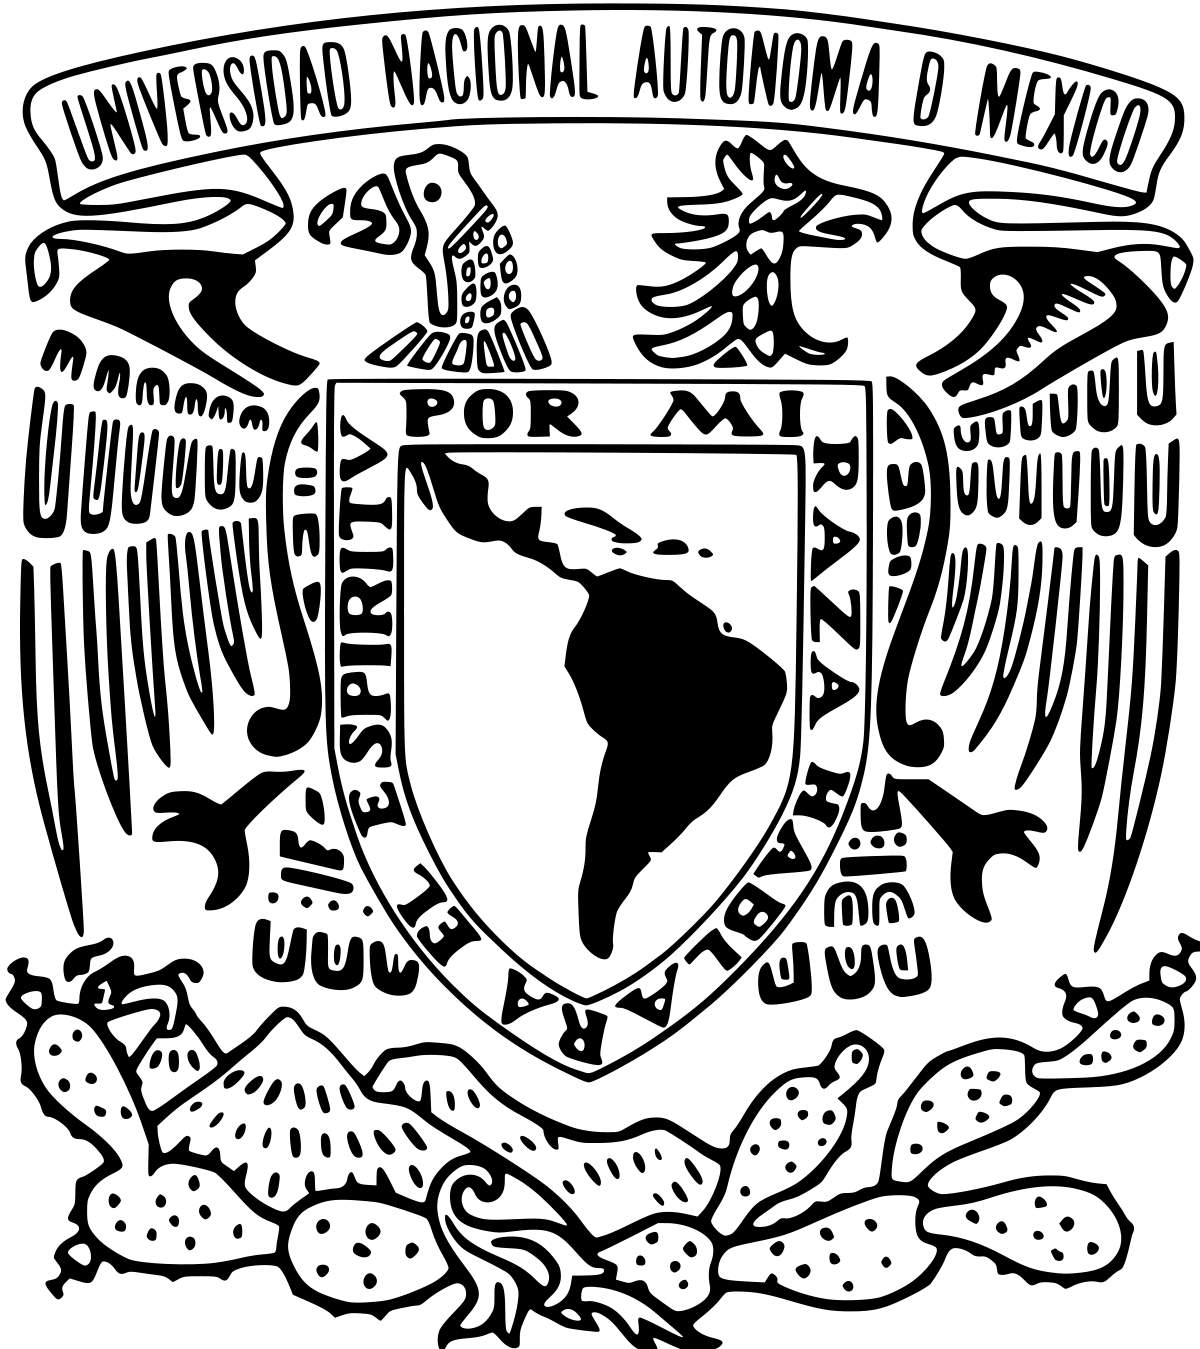
\includegraphics[width=4cm]{Logo_UNAM.png}
			\label{EscudoUNAM}
	   \endminipage
	   \minipage{0.32\textwidth}
			
\includegraphics[height = 4.9cm ,width=4cm]{escudofi_negro.jpg}
			\label{EscudoFI}
		\endminipage
	\end{figure}
	
	\begin{center}
	\vspace{0.8cm}
	\LARGE
	UNIVERSIDAD NACIONAL AUTÓNOMA DE MÉXICO 
	
	\vspace{0.8cm}
	\LARGE
	FACULTAD DE INGENIERÍA
	
	\vspace{1.7cm}	
	\Large
	\textbf{Proyecto Final}

	\vspace{1.3cm}
	\normalsize	
	PRESENTA \\
	\vspace{.3cm}
	\large
	\textbf{Martínez Ruiz Denisse \\ Martínez Silva Frida Estefanía}
	
	\vspace{1.3cm}
	\normalsize	
	PROFESOR \\
	\vspace{.3cm}
	\large
	\textbf{Fernando Arreola Franco}
	
	\vspace{1.3cm}
	\normalsize	
	ASIGNATURA \\
	\vspace{.3cm}
	\large
	\textbf{Bases de Datos}
	
	\vspace{1.3cm}
	25 de Enero de 2021
	\end{center}
	\newpage
	

	\paragraph{INTRODUCCIÓN:}
	\justifying
	 \paragraph{Se planea diseñar un sistema de control para una papelería, basándonos en las técnicas aprendidas a lo largo del curso de la materia de Bases de Datos, estos temas son: MER, MR, creación de tablas, llenado de las mismas, entre otros. \\ \\
     Para comprender el problema de este proyecto debemos identificar cuáles son sus entidades, atributos de cada una de ellas y la relación entre estas, para proceder con el diseño incluyendo todas las restricciones que se piden, en donde entran los respectivos modelos.\\ \\
     Posterior a esto realizamos la normalización de las tablas, donde verificamos que no hubiera grupos de repetición, dependencias parciales, y dependencias transitivas.\\ \\
	 Para la creación de la base de datos y creación de tablas, se hizo uso de PgAdmin, una herramienta para la administración de bases de datos propia de PostgreSQL, así como para su llenado y las diversas operaciones y consultas que debíamos realizar.\\ \\
     Finalmente el diseño de la página web, creada en html, php y css; se optó por utilizar la aplicación XAMPP para el servidor de la pagina web ya que cuenta con Apache y nos permite alojar nuestra pagina de manera local, para posteriormente con lineas de código dentro del mismo HTML lograr conectarla a la base de datos..}
	 
	 \paragraph{PLAN DE TRABAJO:}
	 \justifying
	 \paragraph{Para el plan de trabajo utilizamos la herramienta Trello, la cual nos permite seleccionar los trabajos a realizar, dividiéndolo en fases de diseño, modelos, creación de tablas, llenado de información, página web, documentación y por último exposición.}
	 \paragraph{Esta herramienta es útil, pues podemos especificar fechas, links de páginas donde se trabajaría cada etapa, adicional a esto se tuvieron juntas donde se aseguraba que todos estuviéramos de acuerdo con los diseños elaborados.}
	 \begin{center}
	    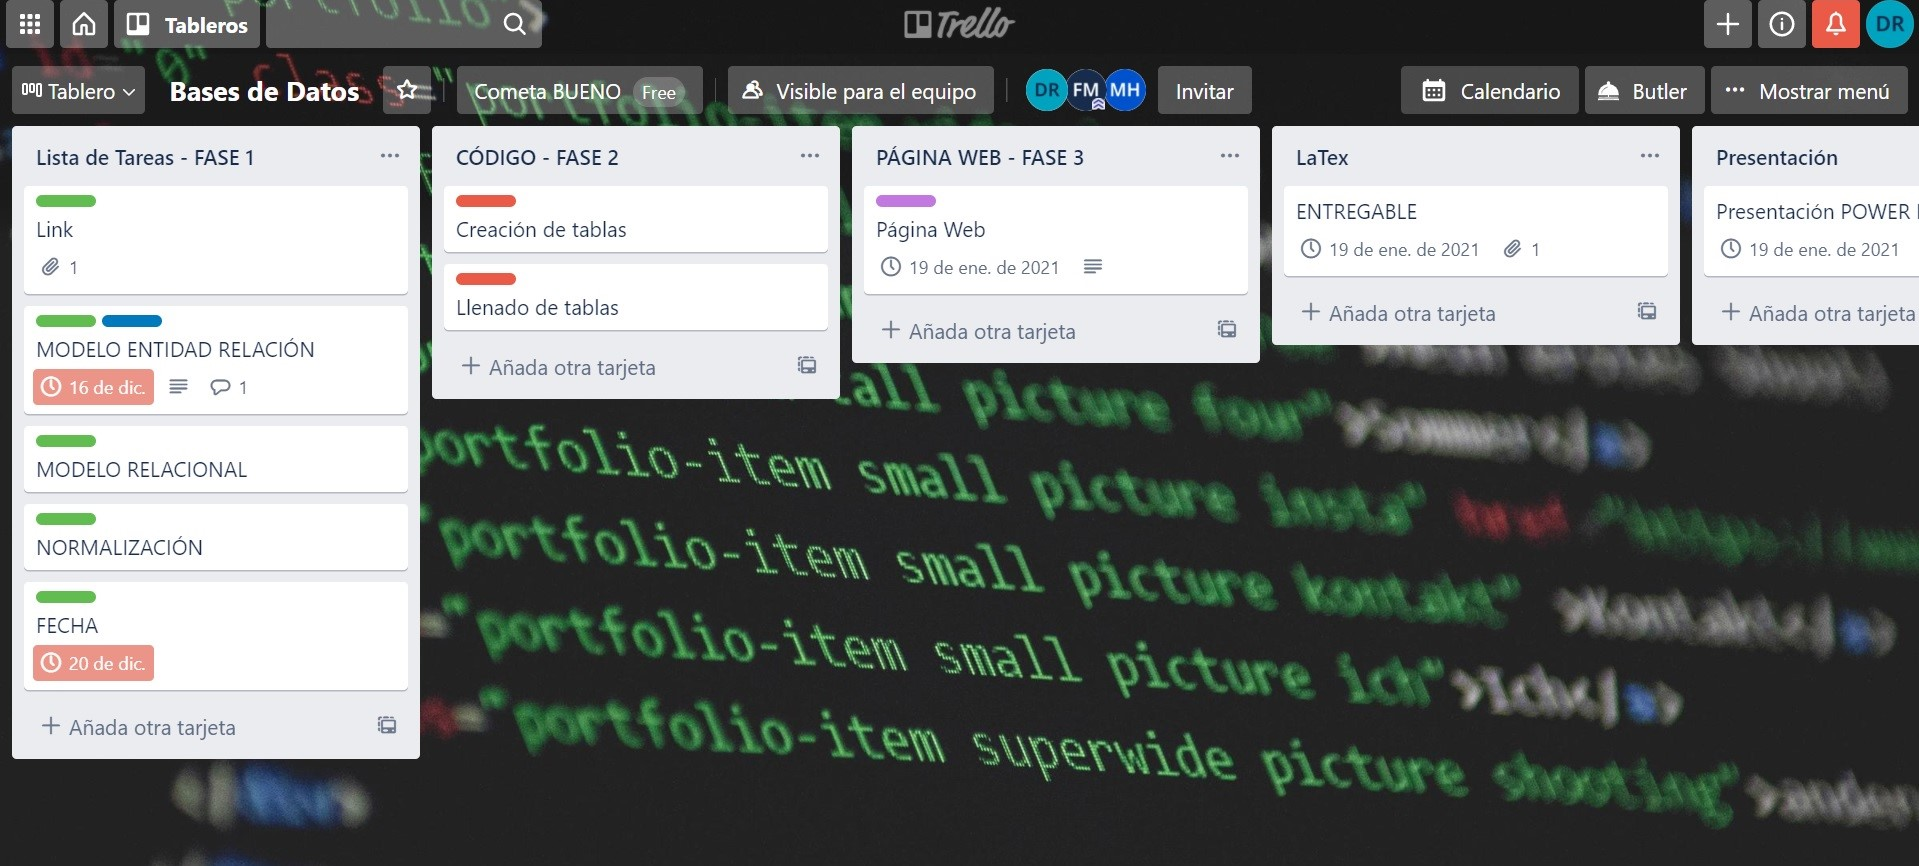
\includegraphics[height= 8cm, width=15cm]{trello.jpg}
	     \caption{Evidencia Trello}
	     \label{Trello}
	 \end{center}
	 \paragraph{Se empleó draw.io para el diseño de los modelos, ya que nos permite el trabajo en equipo de manera remota, su almacenamiento es en la nube y a su vez integra la plataforma de Google Drive. Mientras que para la redacción del presente documento se optó por la herramienta Overleaf, que al igual que la anterior permite el trabajo en equipo remoto y la compilación del mismo desde el navegador.}
	 \paragraph{
	 \begin{tabular}{|r|l|}
	        \hline
	      Integrante & Actividad  \\ \hline
	      Denisse & Diseño de la página web, creación de scripts de la base de datos, programación \\
	       & de funciones como lo fue obtención de utilidad, obtención de número de ventas  \\
	       &  según fecha o fechas,  diseño de MR, MER.\\ \hline
	      Frida &   Diseño de MR y MER, creación de scripts de llenado de información\\ & y programación (stock, generación de vista de factura), diseño de pagina web,\\ & redacción del presente documento.\\
	      \hline
	 \end{tabular}}
    \justifying
	 \paragraph{DISEÑO:}
	\paragraph{Fase Uno:\\\\
	Nos enfocamos en entender todos los requisitos para la resolución del proyecto. La fase fue divida en tres etapas, modelo entidad relación, modelo relacional y normalización.\\\\
	MODELO ENTIDAD RELACIÓN: En está etapa se trabajó el modelo entidad relación, respetando los tipos de atributos, las entidades, relaciones y atributos en relaciones, se tomaron ciertas consideraciones del problema las cuales se proyectan en este modelo. }
    \paragraph{Una vez realizado el MER procedemos con el MR.}
     \begin{figure}[h]
	     \centering
	   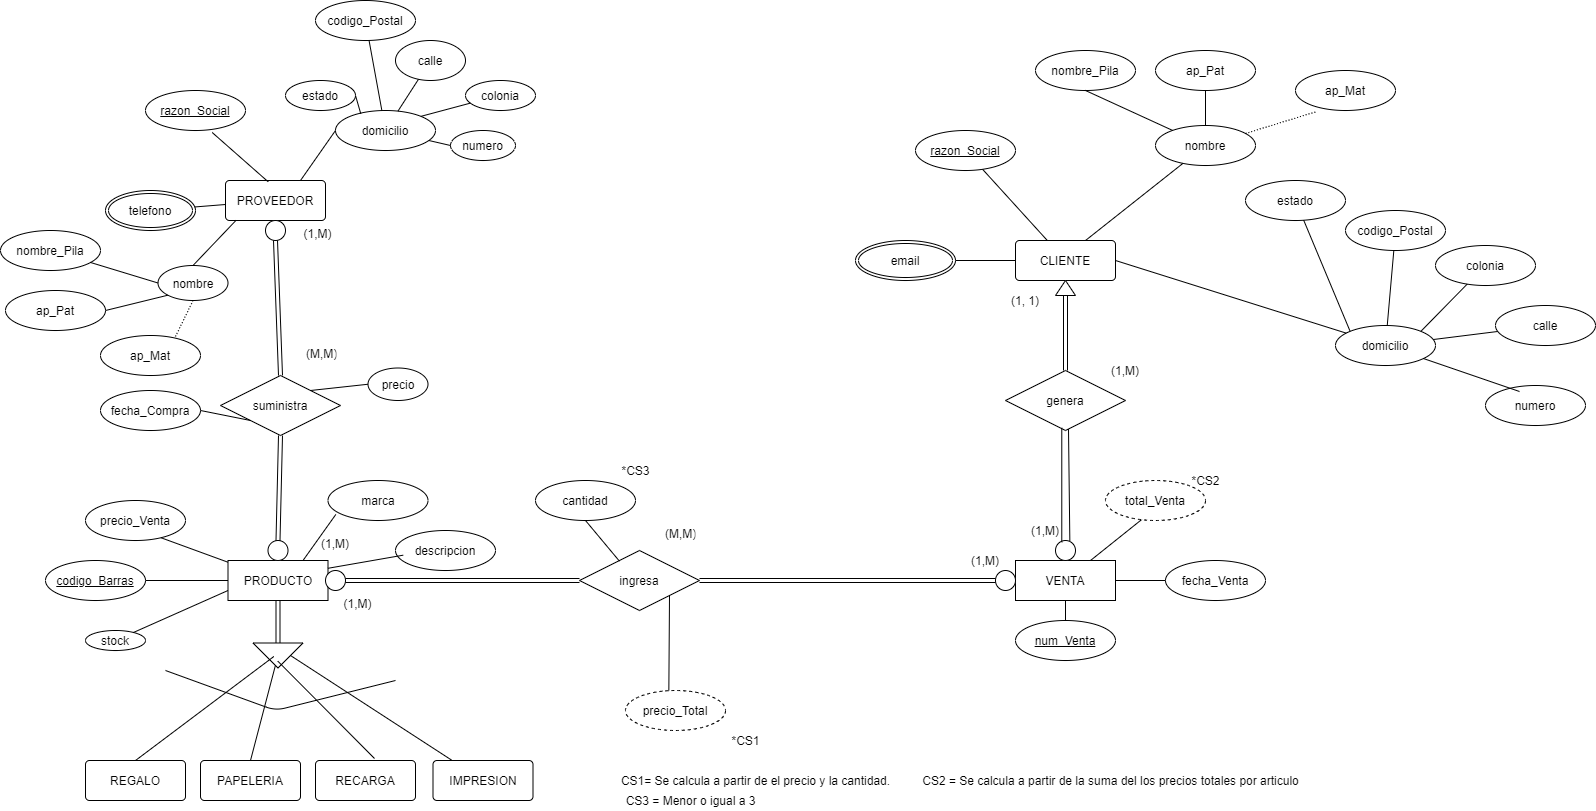
\includegraphics[height= 11cm, width=17cm]{MER1.png}
	   \caption{Modelo Entidad Relación}
	     \label{MER}
	 \end{figure}
	 \paragraph{MODELO RELACIONAL: A partir del modelo anterior se obtiene el modelo relacional siguiendo una serie de reglas, obtuvimos el modelo intermedio el cual se muestra a continuación. }

	 
	 \paragraph{PROVEEDOR=\{razon\_Social varchar (50) (PK), nombre varchar \(50\), ap\_Pat varchar (80), ap\_Mat varchar(80), calle varchar (40), numero smallint, colonia varchar (40) codigo\_Postal int, estado varchar (40)\}\\
	 TELEFONO:\{ razon\_Social varchar(50)(FK)(PK), telefono bigint (PK)\}\\
	 SUMINISTRA:\{[razon\_Social\_Proveedor varchar(50), codigo\_Barras varchar(15)](FK)(PK), precio\_Compra int, fecha\_Compra date\}\\
	 PRODUCTO:\{codigo\_Barras varchar(15) (PK), stock smallint, precio\_Venta int, marca varchar(40), tipo\_Producto varchar(15) \}\\
	 DETALLE:\{[codigo\_Barras varchar(15), no\_Venta text](PK)(FK), cantidad numeric, precio\_Subtotal int\}\\
	 VENTA:\{no\_Venta text (PK), fecha\_Venta date, total\_Venta int, razon\_Social\_Cliente varchar (50) (FK)\}\\
	 CLIENTE:\{razon\_Social varchar (50) (PK), nombre varchar \(50\), ap\_Pat varchar (80), ap\_Mat varchar(80), calle varchar (60), numero smallint, colonia varchar (60) codigo\_Postal int, estado varchar (40)\}\\
	 EMAIL :\{[email varchar(80), razo\_Social\_Cliente varchar(50)(FK)](PK)\}
	 }

    \paragraph{Posterior a esto elaboramos el modelo relacional, en el cual es mucho más sencillo visualizar la relación entre cada una de las entidades.}

	 \paragraph{Una vez hecho esto continuaos con la normalización, esto, para verificar que cumpla con cada una de las condiciones que se pretende.}
	  \begin{figure}[h]
	     \centering
	   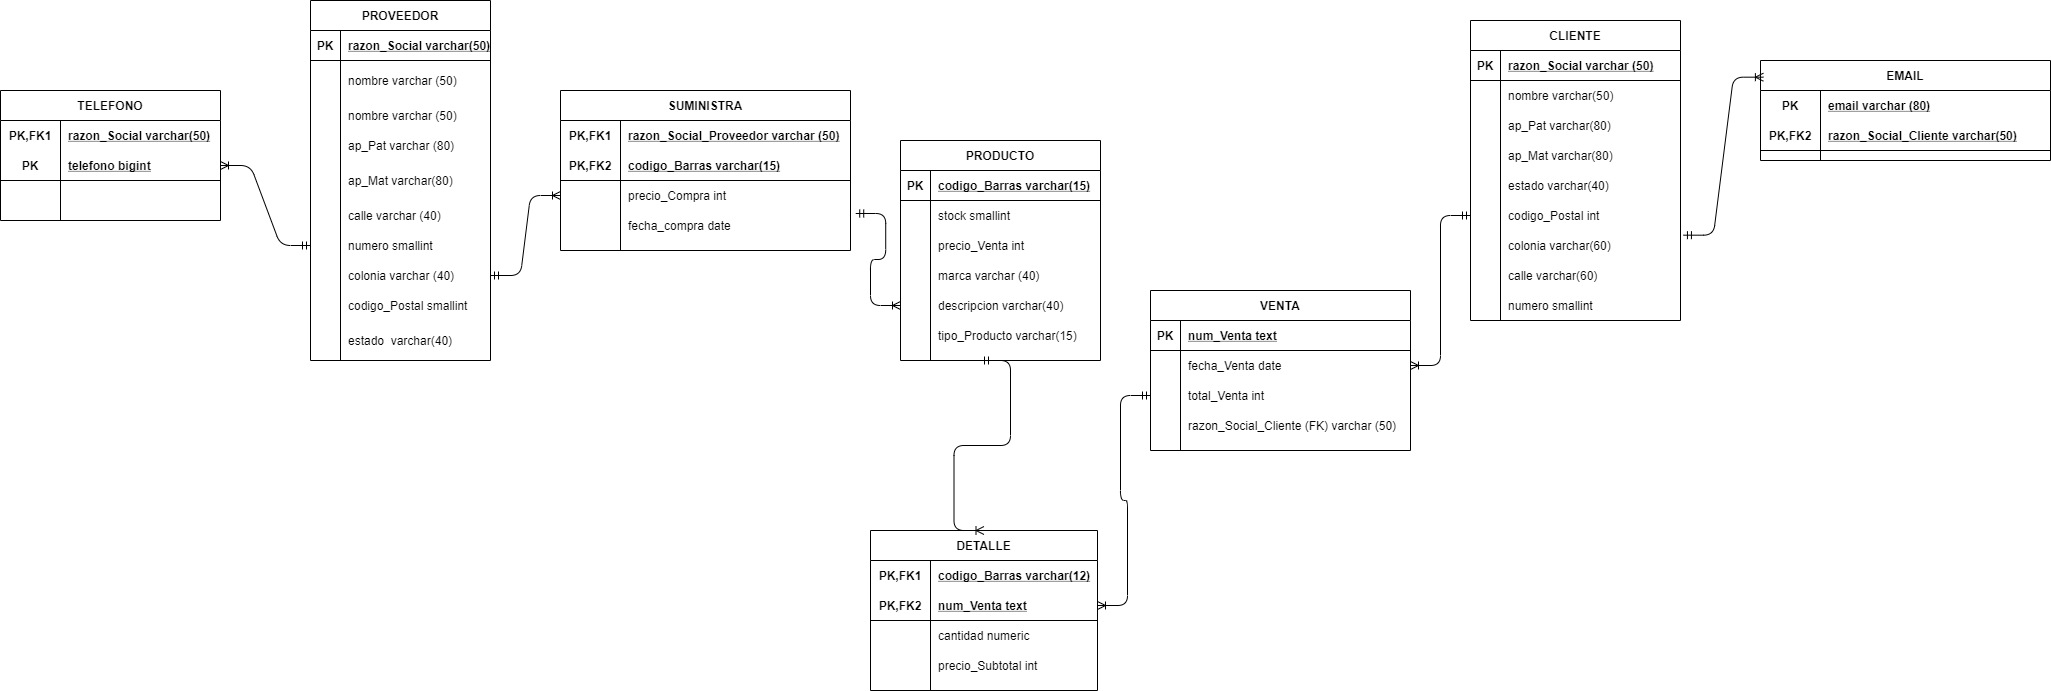
\includegraphics[height= 5cm, width=17cm]{MR.png}
	   \caption{Modelo Relacional}
	     \label{Inter}
	 \end{figure}
	 \paragraph{NORMALIZACIÓN }

	 \paragraph{1FN: En la primer forma normal verificamos que no existan grupos de repetición, así como valores atómicos. Nuestras tablas anteriores no contienen grupos de repetición y cada uno de sus valores es atómico, por lo tanto cumple con la 1FN.\\\\
	 2FN: La segunda forma normal nos dice que una relación se encuentra en segunda formal si no existen dependencias parciales, aquellas en las que un atributo dependa de únicamente de una llave en una llave compuesta. Las tablas que deberíamos de estar verificando sería SUMINISTRA y DETALLE, al hacer el análisis no existen dependencias parciales.\\\\
	 3FN:Por último en esta forma normal buscamos eliminar las dependencias transitivas en la cual un atributo de nuestra relación depende de otro atributo y a la vez ese mismo atributo dependa de una llave primaria. Notamos que ninguna de nuestras tablas tenemos dependencias transitivas.}
	 	 	  \paragraph{
	  \begin{center}
	     \centering
	   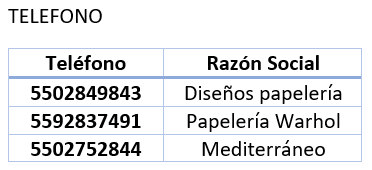
\includegraphics[height= 3cm, width=5cm]{telefono.PNG}
	   \caption{Tabla Teléfono}
	     \label{Inter}
	 \end{center}
	 	  \begin{center}
	   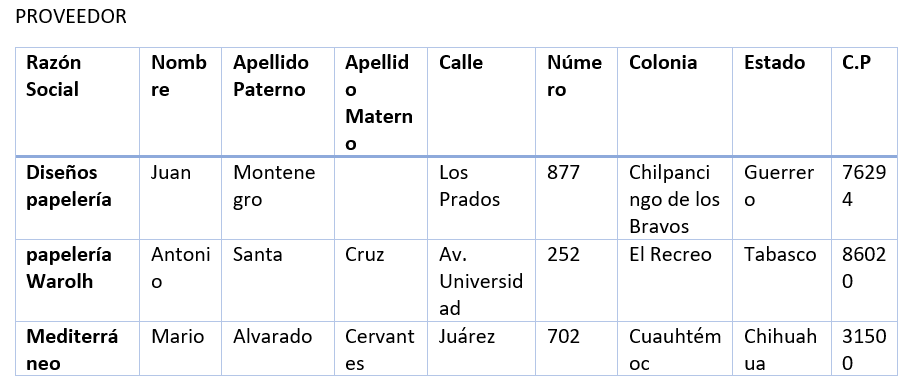
\includegraphics[height= 5cm, width=15cm]{PROVEEDOR.PNG}
	   \caption{Tabla Proveedor}
	     \label{Inter}
	 \end{center}
	   \begin{center}
	   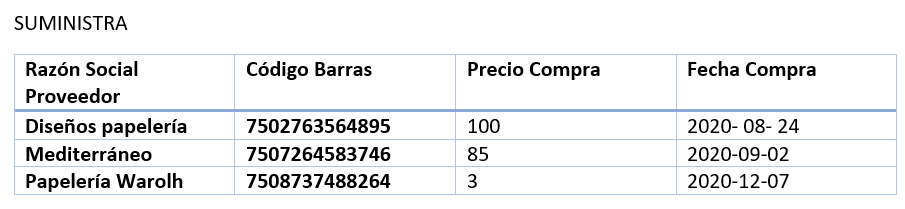
\includegraphics[height= 4cm, width=15cm]{suministra.PNG}
	   \caption{Tabla Suministra}
	     \label{Inter}
	 \end{center}	 
	   \begin{center}
	   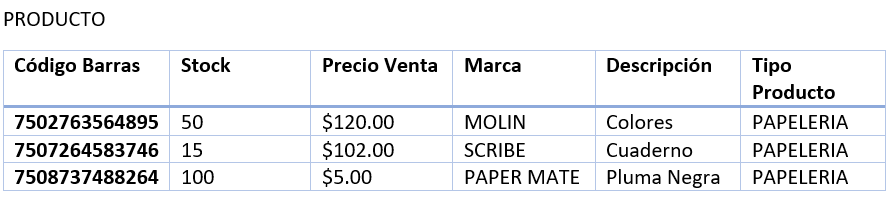
\includegraphics[height= 4cm, width=15cm]{producto.PNG}
	   \caption{Tabla Producto}
	     \label{Inter}
	 \end{center}
        \begin{center}
	   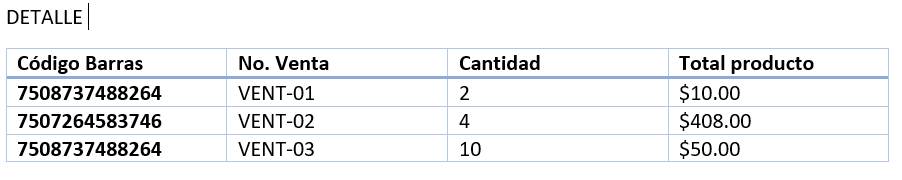
\includegraphics[height= 4cm, width=15cm]{detalle.PNG}
	   \caption{Tabla Detalle}
	     \label{Inter}
	 \end{center}
	  \begin{center}
	   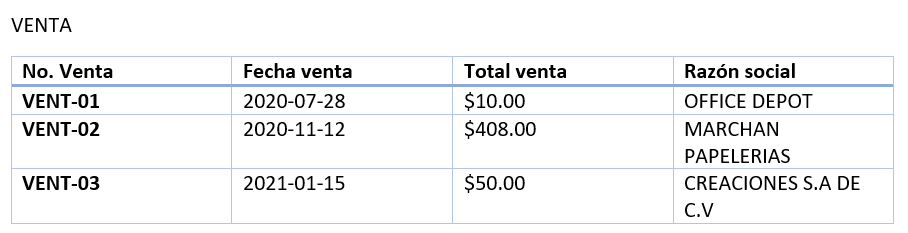
\includegraphics[height= 4cm, width=15cm]{venta.PNG}
	   \caption{Tabla Venta}
	     \label{Inter}
	 \end{center}
	 \begin{center}
	   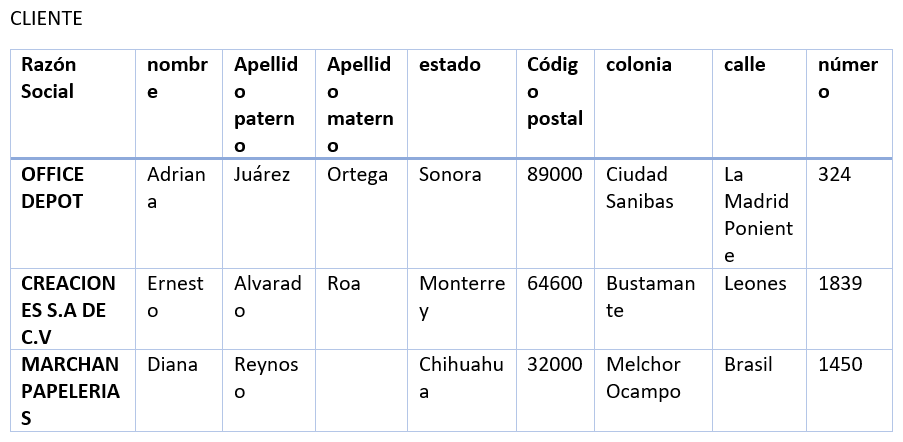
\includegraphics[height= 5cm, width=15cm]{cliente.PNG}
	   \caption{Tabla Cliente}
	     \label{Inter}
	 \end{center}
	  \begin{center}
	   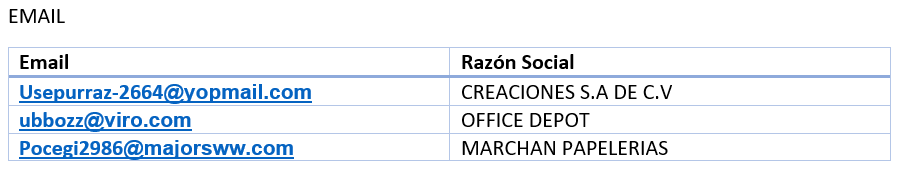
\includegraphics[height= 4cm, width=10cm]{email.PNG}
	   \caption{Tabla Email}
	     \label{Inter}
	 \end{center}
	 }
    \paragraph{IMPLEMENTACIÓN}
	 \paragraph{Se describen cada uno de los stores procedures, triggers, funciones que se implementan en la base de datos para cumplir con los requerimientos dados.}
	 
	 \paragraph{Nuestro primer requerimiento es la obtención de la utilidad dado un codigo de barras. Para ello se hizo uso de una función, en el caso de PostgreSQL, la función se puede crear o remplazar. Para ello se necesita el comando''CREATE OR REPLACE FUNCTION'' seguido del nombre de la función, la cual recibe como parámetro el código de barras, seguido del comando ''RETURNS'' y el tipo de dato que retornará, para este caso en particular, un entero. Dentro del cuerpo de la función hacemos un''SELECT'' el cual mediante un ''INNER JOIN'' entre la tabla PRODUCTO y SUMINISTRA nos devuelve la utilidad del número de barras que estamos ingresando. Se decidió utilizar lenguaje SQL ( lenguaje universal) ya que unicamente se haran consultas.}
	 
	 \paragraph{En cuanto al segundo requerimiento tenemos el que devuelve la cantidad vendida dada una fecha o un periodo de tiempo. Para esto hicimos uso de dos funciones una que recibe únicamente un parámetro y la otra dos, en cuanto a los parámetros que recibe son la fecha o fechas en las que se desea conocer la cantidad que se vendió, y nos devolverá un entero. En la función anterior se explican los comandos utlizados para el tipo de retorno y la creación de la función. Pasamos a lo que realizara la función, es un ''select'' que realiza un ''FULL JOIN'' entre la base DETALLE e INGRESA comparando los registros en los cuales aparece la fecha o periodo de fechas ingresadas haciendo una suma de todas esas cantidades. }
	 
	 \paragraph{Para los productos de los cuales menos de 3 en stock, igualmente se ocupa una función, la diferencia de esta, es que no recibe ningún parámetro y devuelve una tabla que contendrá el nombre de nuestros productos que tengan menos de 3 en stock haciendo uso de un WHERE para el filtrado de datos.}
	 
	 \paragraph{El siguiente requerimiento es generar una vista automática de una factura. Para ello necesitaremos de una función que dado un número de venta nos genere la factura de dicha venta, para esto se consideraron los datos necesarios de una factura como fecha, numero de factura, información del cliente, detalles de la venta y total. Se decidió hacer uso de un ''RAISE NOTICE'' para generar los datos como texto plano y no en una tabla.}
	 
	 \paragraph{El índice se decidió utilizar un indice de tipo B-Tree en la columna stock de la tabla PRODUCTO, ya que acepta operaciones como >, <, =, entre otros, y esta columna, puesto se ocupará en más funciones.}
	 
	 \paragraph{Por último contamos con un procedimiento almacenado que se ocupará para insertar en la tabla DETALLE. Este recibirá tres valores, el código de barras, numero de venta y cantidad, al iniciar hace un INSERT de los datos en la tabla DETALLE y se dipara el trigger que actualiza el total por producto y total de venta, posterior realiza un select para obtener el stock de dicho producto y compararlo con la cantidad vendida. Si el stock del producto es mayor a la cantidad, se procede a ejecutar un COMMIT, después consulta nuevamente el stock y verifica si es menor a 3 pero mayor a 0, notifica que el producto está próximo a agotarse, y en caso de que sea 0 hace un ROLLBACK a la transacción.}

    \paragraph{PRESENTACIÓN:}
    \paragraph{La modalidad seleccionada de conexión entre la base y la página web es cliente-servidor mediante PHP. 
    \\PHP es un lenguaje de código abierto muy popular especialmente adecuado para el desarrollo web y que puede ser incrustado en  HTML, donde el código es ejecutado en el servidor, generando HTML y enviándolo al cliente. }
    \paragraph{La conexión de base de datos se hace mediante líneas de código en donde se comparte código de php, combinado con PL/PgSQL (el que utilizamos en la base de datos). Para alojar la base de datos en un servidor local se hace uso de XAMPP, distribución de Apache completamente gratuita y fácil de instalar.\\\\
    A continuación se muestra un diagrama que ejemplifica de manera gráfica la conexión.}
    
      \begin{center}
	   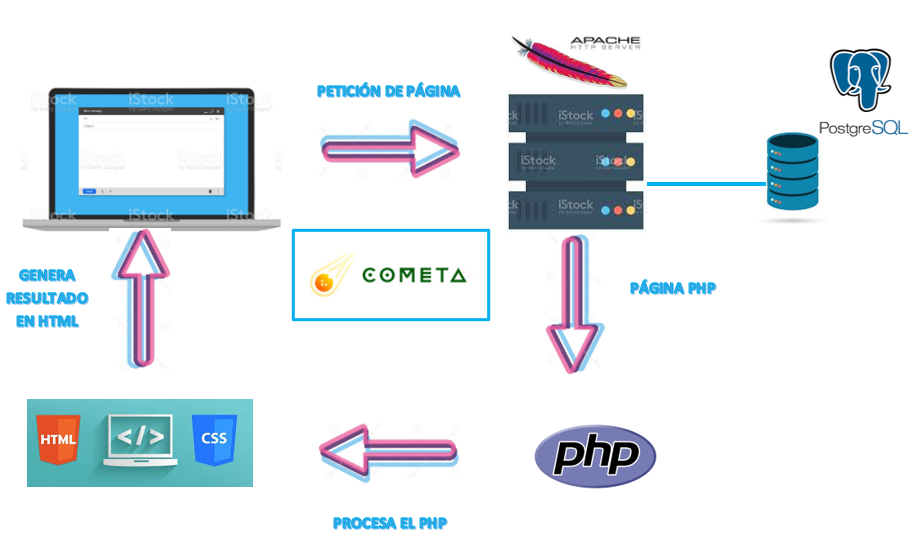
\includegraphics[height= 6cm, width=14cm]{conexion.PNG}
	   \caption{Diagrama de conexión}
	     \label{Inter}
	 \end{center}
    
    \paragraph{CONCLUSIONES:}
    \paragraph{Martínez Ruiz Denisse: El proyecto fue un reto personal, aplicar todos esos conceptos no solo los aprendidos desde el primer día de clases, también aquellos que cómo próximo ingeniero en sistemas deberías de conocer, como lo fue la creación de la página web, y el almacenamiento de la misma en un servidor. El hecho de delegar responsabilidades y confiar en tu equipo fue un punto medular. Lo más complicado fue la elaboración de los triggers, pero con revisión de diversas fuentes finalmente se consiguió. Otro punto que nos atraso, fue una parte de la conexión entre la pagina y la base, específicamente la de inserción de productos, ya que primero se debe ingresar información a la tabla VENTA y esta te genera el número de venta que se debe ingresar a la tabla DETALLE, por lo demás fue un proyecto extenso, y al ser únicamente dos integrantes la carga de trabajo era mucho mayor. }
    \paragraph{Martínez Silva Frida Estefanía: La materia de bases de datos ha sido una de las cuales más temor me ha causado, pues en semestres anteriores no tuve buena experiencia con ella, sin embargo, he aprendido bastante y me ha ayudado a forjar conocimientos que previamente no me habían quedado del todo claros. 
    \\Para este proyecto ha sido una constante búsqueda e indagación de información, ya que, los requerimientos dados, llevaban a mi parecer una complejidad mayor. Uno de los problemas que tuvimos fue a la hora de calcular tanto el subtotal y total de nuestra venta, pues no lo calculaba de la manera en que nosotras queríamos, después de días de pensar y buscar encontramos el error. Así mismo con la página web, un pequeño error puede hacer que todo cambie y que tu cabeza se confunda más. 
    \\Por último, cabe destacar que todo lo que se vio en clase y más, fue aplicado en este proyecto, al usar herramientas de organización como Trello, de diseño como draw.io, para la base pgAdmin y la Página web apoyarnos tanto de PHP como HTML, fue toda una experiencia que espero más adelante podamos aplicar tanto en materias futuras como en el campo laboral.}
    
\end{document}